% Section 7 — Discussion and Conclusion

% ──────────────────────────────────────────
%  Figure: Cross-Model Heatmap (placed here for right-column [t] on p8)
% ──────────────────────────────────────────
\begin{figure}[t]
\centering
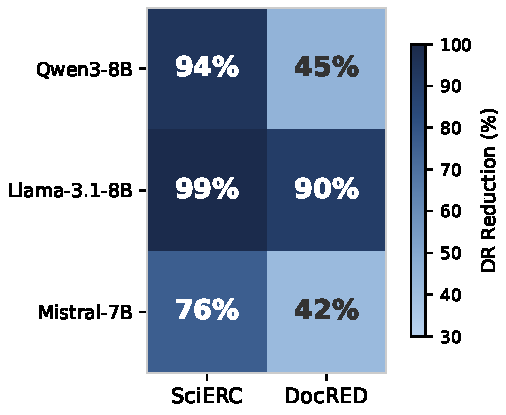
\includegraphics[width=0.75\columnwidth]{figures/fig_crossmodel_heatmap.pdf}
\caption{DR reduction (\%) across 3 models $\times$ 2 datasets (zero-shot S1). Calibrated models (Qwen, Llama) achieve $\geq$90\% on SciERC; DocRED's higher $\bar{\kappa}$ reduces effectiveness. Full violation breakdown in Table~\ref{tab:cross-model} (Appendix~\ref{app:cross-model-zs}).}
\label{fig:crossmodel-heatmap}
\end{figure}

Neither layer alone suffices: grammar-only achieves 3\% DR reduction, semantic-only 24\%, but their composition yields 94\%, an enabling dependency that weakens at scale (84\% at 70B).
This non-additive interaction arises because the grammar layer provides a structured prerequisite: by restricting relation tokens to $\mathcal{R}$ and entity type tokens to $\mathcal{E}$, it ensures the semantic layer receives well-formed inputs on which domain/range lookups can operate.
Without grammar-enforced vocabulary membership, the semantic layer cannot reliably identify which relation governs a given type position.

OntoCoDec composes both layers, reducing DR to $\leq$\,0.21\% across model families and datasets ($\pm$0.3\,pp R-F1).
The residual DR$\to$CF conversion is a severity downgrade rather than an error introduction: DR violations produce ontology-invalid triples that corrupt downstream knowledge graphs and require re-extraction, while CF violations (cross-triple type inconsistency) preserve individually valid triples and are resolvable via beam search or post-hoc reranking.
Beam $k{=}4$ achieves near-zero violations at 8B, making generative IE reliably schema-compliant.
